\label {fs-short-intro}

%Refs:~\cite{Akidau:2013:MFS:2536222.2536229, Carbone:2017:SMA:3137765.3137777, Li2011, Li:2008:OPN:1453856.1453890, Murray:2013:NTD:2517349.2522738, Stonebraker:2005:RRS%:1107499.1107504, Zaharia:2012:DSE:2342763.2342773, we2018seim}

Exactly-once semantics even in a presence of failures is a desired property for stream processing systems~\cite{Akidau:2013:MFS:2536222.2536229}. One way to achieve it is to snapshot operations states atomically with respect to producing output~\cite{Carbone:2017:SMA:3137765.3137777} and to restart processing from the last successful snapshot on recovery. However, in this case, latency cannot be less than the period of snapshotting. Another attractive approach is to make system idempotent, i.e., to ensure that input replay does not lead to duplicates on output. Google's MillWheel achieves idempotence by persistently logging each input item~\cite{Akidau:2013:MFS:2536222.2536229}. This technique called {\em strong productions} limits the throughput of the operations by the throughput of logs storage. On the other hand, idempotence can be easily achieved if computations are deterministic, i.e., several runs on the same data produce the same result. In this case, extra data can be simply filtered out at the system entrance. {\em Discretized streams} technique is based on {\em RDD} model and provides for deterministic computations~\cite{Zaharia:2012:DSE:2342763.2342773}. However, it implies buffering on input and latency higher than approximately one second~\cite{Qian:2013:TRS:2465351.2465353}. IOP and OOP approaches shift buffer from system entry to operations~\cite{Li:2008:OPN:1453856.1453890}. OOP method can reduce latency, but buffering before each order-sensitive operation is still inappropriate for many applications~\cite{Zacheilas:2017:MDS:3093742.3093921}. The scheme of approaches for exactly-once is shown in Figure~\ref{approaches}.

\begin{figure}[ht]
  \centering
  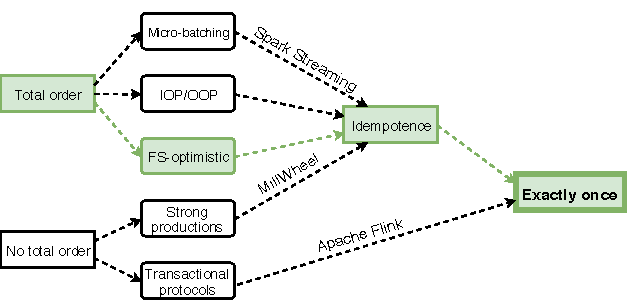
\includegraphics[width=0.47\textwidth]{pics/intro-approaches}
  \caption{The approaches for exactly-once processing}
  \label {approaches}
\end{figure}

In this work, we introduce the OOP-based architecture that allows us to leave only one buffer per computational pipeline while achieving determinism, and therefore, exactly-once. Our speculative approach is based on the special limited set of operations that are enough to express any stateful transformation and can be implemented in an optimistic manner. Such behavior is achieved using {\em drifting state} that allows a state to flow along a stream. In sections~\ref{fs-short-model} and~\ref{fs-short-discussion} we explain the main ideas behind our model. In~\ref{fs-short-experiments} we demonstrate that our approach can significantly outperform an industrial alternative within a real-life problem. 